\section{Thiết kế và triển khai quy trình trích xuất, biến đổi, nạp dữ liệu (ETL)}

\subsection{Kiến trúc tổng thể hệ thống ETL}

Hệ thống ETL (Extract - Transform - Load) được thiết kế là trung tâm điều phối dữ liệu của toàn bộ dự án Traffic Data Warehouse. Kiến trúc này không chỉ đơn thuần là việc di chuyển dữ liệu, mà còn là quá trình chuẩn hóa không gian - thời gian, làm giàu dữ liệu bằng AI và tối ưu hóa cấu trúc lưu trữ để phục vụ các truy vấn phân tích phức tạp.

\subsubsection{Mục tiêu và Nguyên tắc thiết kế kiến trúc}

Hệ thống được xây dựng dựa trên các nguyên tắc thiết kế hiện đại nhằm đảm bảo tính ổn định và khả năng bảo trì lâu dài:

\begin{itemize}
    \item \textbf{Tính Module hóa (Modularity):} Toàn bộ quy trình được chia nhỏ thành các Pipeline riêng biệt: Dimension Pipeline, Mock Data Pipeline và Fact Pipeline. Cách tiếp cận này giúp cô lập lỗi và cho phép thực thi từng phần dữ liệu độc lập theo nhu cầu.
    \item \textbf{Tính nhất quán dữ liệu (Data Atomicity):} Sử dụng các cơ chế Transaction và kỹ thuật "Upsert" (Update or Insert) thông qua câu lệnh \texttt{ON CONFLICT} để đảm bảo dữ liệu không bị trùng lặp và luôn duy trì trạng thái mới nhất ngay cả khi quy trình ETL bị gián đoạn.
    \item \textbf{Tính toàn vẹn không gian (Spatial Integrity):} Mọi dữ liệu giao thông từ API đều được ánh xạ (Mapping) chính xác vào hệ hạ tầng tĩnh (Nodes, Segments) dựa trên các thuật toán hình học của PostGIS.
    \item \textbf{Khả năng mở rộng (Scalability):} Kiến trúc cho phép tích hợp thêm các nguồn dữ liệu mới như cảm biến IoT hoặc camera giao thông chỉ bằng cách bổ sung các module Service mà không cần thay đổi cấu trúc lõi của Pipeline.
\end{itemize}

\begin{figure}[htbp]
    \centering
    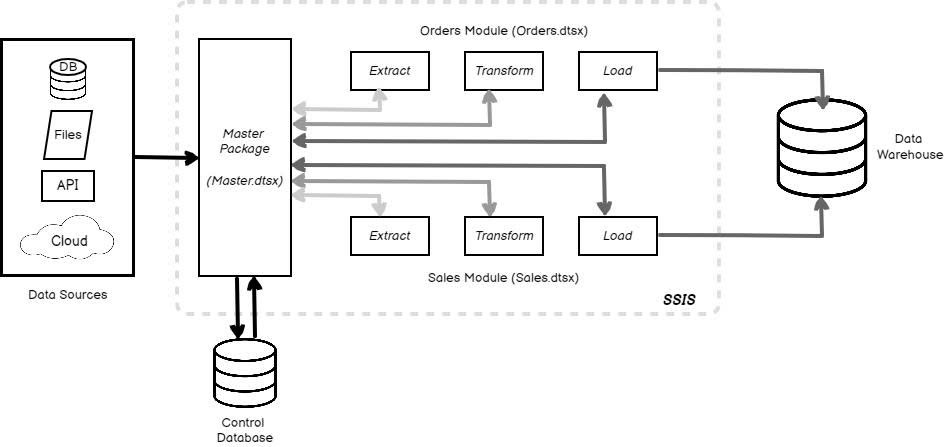
\includegraphics[width=0.8\textwidth]{Images/ETL_01}
    \vspace{6mm}
    \caption{Sơ đồ kiến trúc tổng thể hệ thống ETL}
    \label{fig:etl_01}
\end{figure}

\subsubsection{Mô hình phân lớp chức năng (Functional Layering)}

Kiến trúc ETL được tổ chức thành 4 tầng chức năng chặt chẽ:

\begin{enumerate}
    \item \textbf{Tầng thu thập (Extraction Layer):} Thực hiện kết nối và trích xuất dữ liệu đa nguồn: API thời gian thực (TomTom, OpenWeather), dữ liệu không gian (OpenStreetMap), dữ liệu nhận diện hình ảnh (YOLOv8) và dữ liệu tĩnh (CSV). Sử dụng cơ chế quản lý API Key và tham số hóa để tối ưu số lượng request (Free Tier giới hạn).
    \item \textbf{Tầng biến đổi và làm giàu (Transformation \& Enrichment Layer):} Thực hiện các phép tính toán nghiệp vụ giao thông: quy đổi lưu lượng xe sang đơn vị PCU, tính toán hướng đường (Azimuth) và xác định ranh giới hành chính bằng Spatial Join. Tích hợp mô hình học sâu YOLOv8 để chuyển đổi dữ liệu hình ảnh thô thành dữ liệu số lượng phương tiện định lượng.
    \item \textbf{Tầng lưu trữ đích (Loading Layer):} Nạp dữ liệu vào PostgreSQL. Áp dụng các kỹ thuật quản trị hiệu năng: Đánh chỉ mục không gian GIST, chỉ mục văn bản GIN và phân vùng bảng Fact theo dải thời gian (Range Partitioning).
    \item \textbf{Tầng điều phối và Giám sát (Orchestration Layer):} Sử dụng file trung tâm \texttt{main\_etl.py} kết hợp tham số dòng lệnh \texttt{--mode} để điều khiển luồng chạy. Hệ thống hóa nhật ký vận hành (Logging) để theo dõi trạng thái và thời gian thực thi của từng tác vụ.
\end{enumerate}

\subsubsection{Hạ tầng công nghệ và Thư viện lõi}

Hệ thống tận dụng sức mạnh của hệ sinh thái Python 3.12 để xử lý dữ liệu:

\begin{itemize}
    \item \textbf{Quản trị Cơ sở dữ liệu:} \texttt{psycopg2-binary} cung cấp giao thức kết nối hiệu năng cao tới PostgreSQL.
    \item \textbf{Xử lý Dữ liệu Không gian:} \texttt{OSMnx}, \texttt{GeoPandas} và \texttt{Shapely} là bộ ba công cụ dùng để trích xuất đồ thị giao thông và xử lý các đối tượng hình học phức tạp.
    \item \textbf{Xử lý AI và Thị giác máy tính:} \texttt{ultralytics} (YOLOv8) và \texttt{opencv-python-headless} được sử dụng để xây dựng bộ đếm phương tiện thông minh.
    \item \textbf{Xử lý Logic và API:} \texttt{pandas} cho các thao tác trên bảng dữ liệu lớn và \texttt{requests} để tương tác với các REST API bên ngoài.
\end{itemize}

\begin{figure}[htbp]
    \centering
    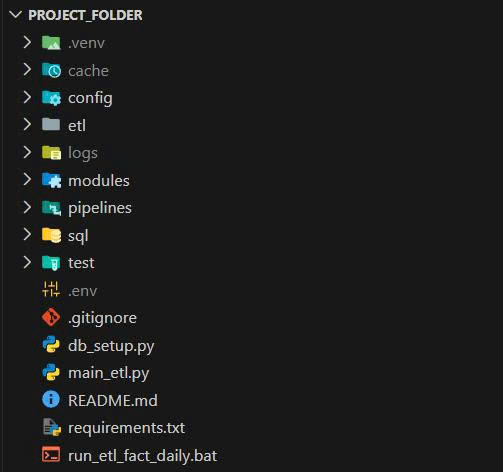
\includegraphics[width=0.6\textwidth]{Images/ETL_02}
    \vspace{6mm}
    \caption{Cấu trúc thư mục dự án hệ thống ETL}
    \label{fig:etl_02}
\end{figure}

\subsubsection{Quản lý cấu hình và Biến môi trường (Environment Configuration)}

Trong một hệ thống ETL hiện đại, việc tách biệt mã nguồn và cấu hình là nguyên tắc cốt lõi nhằm đảm bảo tính bảo mật và khả năng di động của hệ thống. Dự án triển khai cơ chế quản lý biến môi trường thông qua tệp \texttt{.env}, cho phép thay đổi tham số vận hành mà không cần can thiệp vào mã logic.

\begin{itemize}
    \item \textbf{Bảo mật thông tin nhạy cảm:} Các thông tin như thông tin đăng nhập cơ sở dữ liệu (DB\_USER, DB\_PASS) và các khóa truy cập API (TOMTOM\_API\_KEY, OWM\_API\_KEY) được lưu trữ tập trung, tránh việc lộ lọt dữ liệu khi chia sẻ mã nguồn.
    \item \textbf{Tham số hóa phạm vi dữ liệu:} Các biến như ETL\_START\_YEAR và ETL\_END\_YEAR định nghĩa khung thời gian mà hệ thống sẽ khởi tạo dữ liệu nền, giúp dễ dàng điều chỉnh quy mô kho dữ liệu theo nhu cầu phân tích.
    \item \textbf{Công nghệ thực thi:} Hệ thống sử dụng thư viện \texttt{python-dotenv} để tự động tải các biến này vào môi trường chạy của Python ngay khi khởi động.
\end{itemize}

\begin{figure}[htbp]
    \centering
    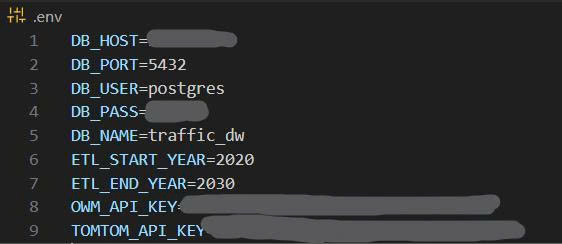
\includegraphics[width=0.7\textwidth]{Images/ETL_03}
    \vspace{6mm}
    \caption{Cấu hình các tham số trong tệp .env}
    \label{fig:etl_03}
\end{figure}

\subsubsection{Quản trị Kết nối và Tài nguyên Cơ sở dữ liệu (Connection Management)}

Để tối ưu hóa việc tương tác với PostgreSQL và đảm bảo tài nguyên hệ thống được giải phóng đúng cách, dự án xây dựng lớp \texttt{DatabaseConfig} tập trung tại \texttt{config/db\_config.py}.

\begin{itemize}
    \item \textbf{Mô hình Singleton hóa kết nối:} Thay vì khởi tạo kết nối rải rác trong từng script, hàm tĩnh \texttt{get\_connection()} cung cấp một phương thức chuẩn duy nhất để thiết lập phiên làm việc với Database.
    \item \textbf{Cơ chế xử lý lỗi kết nối:} Mã nguồn tích hợp khối lệnh \texttt{try-except} để bắt các ngoại lệ khi Database không khả dụng, giúp hệ thống đưa ra thông báo lỗi chi tiết thay vì dừng hoạt động đột ngột.
    \item \textbf{Đóng gói thông số:} Lớp này tự động đọc các biến từ \texttt{.env} (Host, Port, DB Name) để cấu hình tham số cho \texttt{psycopg2}, giúp giảm thiểu sai sót do nhập liệu thủ công trong mã nguồn.
\end{itemize}

\begin{figure}[htbp]
    \centering
    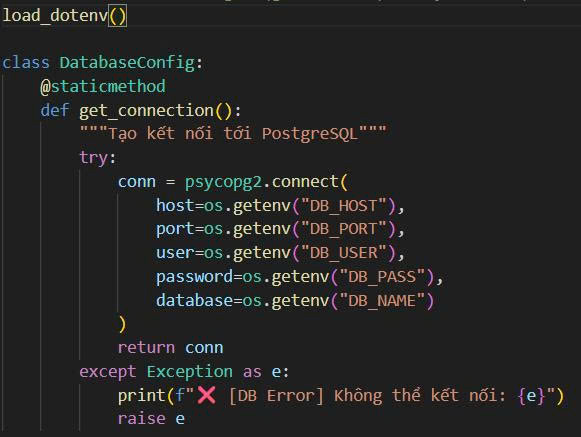
\includegraphics[width=0.8\textwidth]{Images/ETL_04}
    \vspace{6mm}
    \caption{Triển khai lớp DatabaseConfig trong Python}
    \label{fig:etl_04}
\end{figure}

\subsubsection{Cơ chế điều phối đa tầng (Hierarchical Orchestration)}

Để quản lý hàng chục script ETL một cách khoa học, hệ thống triển khai kiến trúc điều phối theo sơ đồ hình cây 3 lớp. Cơ chế này đảm bảo tính tuần tự, quản lý sự phụ thuộc và cho phép khởi chạy linh hoạt theo nhu cầu.

\begin{itemize}
    \item \textbf{Tầng 1: Bộ điều khiển trung tâm (Main Controller):} Tệp \texttt{main\_etl.py} đóng vai trò là điểm vào duy nhất (Single Entry Point) của toàn bộ hệ thống. Sử dụng \texttt{argparse} để tiếp nhận chỉ thị từ người dùng (ví dụ: \texttt{--mode all}, \texttt{--mode fact}). Tại đây, hệ thống thực hiện khởi tạo kết nối Database duy nhất và truyền phiên làm việc (Session) xuống các tầng dưới, giúp tối ưu hóa tài nguyên kết nối.
    \item \textbf{Tầng 2: Các Pipeline nhóm (Group Pipelines):} Nằm trong thư mục \texttt{pipelines/}, các script này đóng vai trò là các "nhóm trưởng" quản lý các thực thể dữ liệu có cùng tính chất:
    \begin{itemize}
        \item \texttt{run\_all\_dims.py}: Điều phối việc nạp dữ liệu nền. Nó đảm bảo các bảng không có khóa ngoại (như dim\_date) phải được chạy thành công trước khi chạy các bảng phụ thuộc (như dim\_segment).
        \item \texttt{run\_all\_facts.py}: Điều phối việc nạp dữ liệu động. Đây là pipeline quan trọng nhất trong vận hành hàng ngày, gọi đồng thời các script nạp Flow, Incident và Weather Impact.
    \end{itemize}
    \item \textbf{Tầng 3: Các Script thực thi nguyên tử (Atomic Scripts):} Đây là lớp cuối cùng nằm trong các thư mục \texttt{etl/infrastructure/}, \texttt{etl/fact/}, v.v.. Mỗi script chỉ đảm nhận một nhiệm vụ duy nhất cho một bảng cụ thể (Single Responsibility Principle), giúp việc gỡ lỗi (Debug) trở nên cực kỳ nhanh chóng.
\end{itemize}

\begin{figure}[htbp]
    \centering
    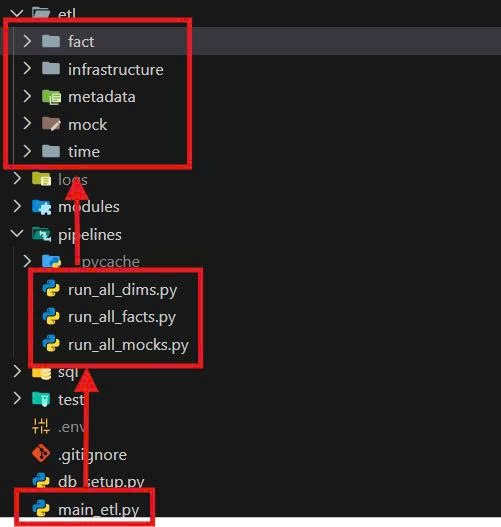
\includegraphics[width=0.6\textwidth]{Images/ETL_05}
    \vspace{6mm}
    \caption{Sơ đồ điều phối Pipeline đa tầng}
    \label{fig:etl_05}
\end{figure}

\subsection{QUY TRÌNH NẠP DỮ LIỆU DIMENSION (DIMENSION ETL PIPELINE)}

Quy trình nạp dữ liệu Dimension được thiết kế để khởi tạo "hệ quy chiếu" cho toàn bộ kho dữ liệu. Pipeline này được điều phối bởi tệp \texttt{pipelines/run\_all\_dims.py}, đảm bảo các bảng độc lập được nạp trước và các bảng có ràng buộc khóa ngoại được nạp sau theo một trình tự logic chặt chẽ.

\subsubsection{Nhóm chiều Thời gian và Lịch (Time \& Calendar Dimensions)}

Dự án triển khai một hệ thống chiều thời gian đa cấp độ, từ mức năm đến mức chi tiết từng phút trong ngày, nhằm hỗ trợ phân tích xu hướng giao thông theo các chu kỳ khác nhau.

\paragraph{Logic xử lý Lịch dương và Lịch âm (Lunar Holiday Logic)}

Việc xử lý dữ liệu thời gian trong bối cảnh giao thông tại Việt Nam đòi hỏi sự chính xác tuyệt đối về các ngày lễ, bởi đây là những thời điểm lưu lượng giao thông biến động cực đoan. Hệ thống triển khai một module chuyên biệt để giải quyết bài toán giao thoa giữa hai hệ thống lịch: Dương lịch (Solar Calendar) và Âm lịch (Lunar Calendar).

\begin{description}
    \item[A. Định nghĩa cấu trúc danh mục ngày lễ (dim\_holiday)] \hfill \\
    Dữ liệu ngày lễ không được nạp cứng mà được quản lý thông qua bảng danh mục \texttt{dim\_holiday} với các thuộc tính linh hoạt:
    \begin{itemize}
        \item \textbf{Cấu trúc lưu trữ:} Mỗi loại ngày lễ được định danh bởi một \texttt{holiday\_code} duy nhất (ví dụ: TET\_HOLIDAY, NATIONAL\_DAY).
        \item \textbf{Phân loại lịch:} Cột \texttt{calendar\_type} xác định quy tắc tính toán là 'SOLAR' hay 'LUNAR'.
        \item \textbf{Quản lý khoảng thời gian:} Thuộc tính \texttt{duration\_days} cho phép xác định một ngày lễ kéo dài bao nhiêu ngày (ví dụ: Tết Nguyên Đán kéo dài 7 ngày), giúp hệ thống tự động sinh dữ liệu cho toàn bộ kỳ nghỉ.
    \end{itemize}
\end{description}

\begin{figure}[htbp]
    \centering
    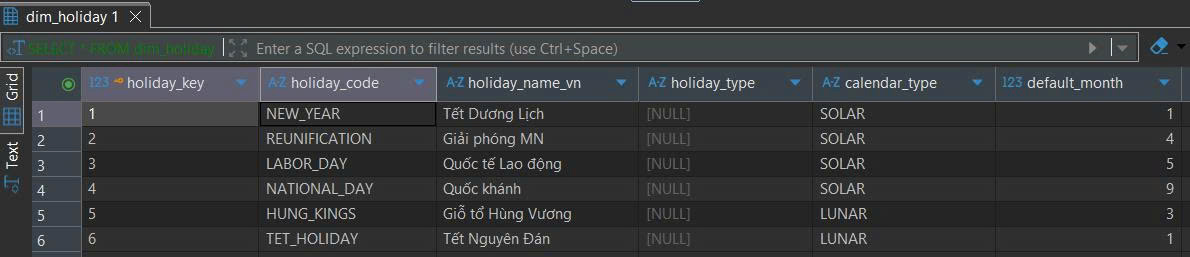
\includegraphics[width=1.0\textwidth]{Images/ETL_06}
    \caption{Dữ liệu cấu hình các ngày lễ trong bảng dim\_holiday}
    \label{fig:etl_06}
\end{figure}

\begin{description}
    \item[B. Thuật toán chuyển đổi và tính toán ngày lễ Âm lịch] \hfill \\
    Do đặc thù các ngày lễ Âm lịch không cố định theo ngày Dương lịch qua từng năm, hệ thống triển khai quy trình chuyển đổi động:
    \begin{itemize}
        \item \textbf{Tích hợp thư viện chuyên dụng:} Sử dụng thư viện \texttt{lunarcalendar} với các lớp \texttt{Converter} và \texttt{Lunar} để thực hiện phép toán chuyển đổi hệ tọa độ thời gian.
        \item \textbf{Vòng lặp tính toán:} Với mỗi năm trong cấu hình \texttt{ETL\_START\_YEAR} đến \texttt{ETL\_END\_YEAR}, hệ thống khởi tạo đối tượng \texttt{Lunar(year, month, day)} dựa trên ngày lễ định nghĩa. Sau đó, hàm \texttt{Converter.Lunar2Solar} sẽ trả về đối tượng ngày Dương lịch tương ứng.
        \item \textbf{Logic đặc thù cho Tết Nguyên Đán:} Riêng đối với mã \texttt{TET\_HOLIDAY}, hệ thống áp dụng logic lùi 1 ngày (\texttt{timedelta(days=1)}) từ mùng 1 Tết để tính toán chính xác ngày "30 Tết", đảm bảo kỳ nghỉ lễ được bắt đầu đúng thực tế văn hóa Việt Nam.
    \end{itemize}
\end{description}

\begin{figure}[htbp]
    \centering
    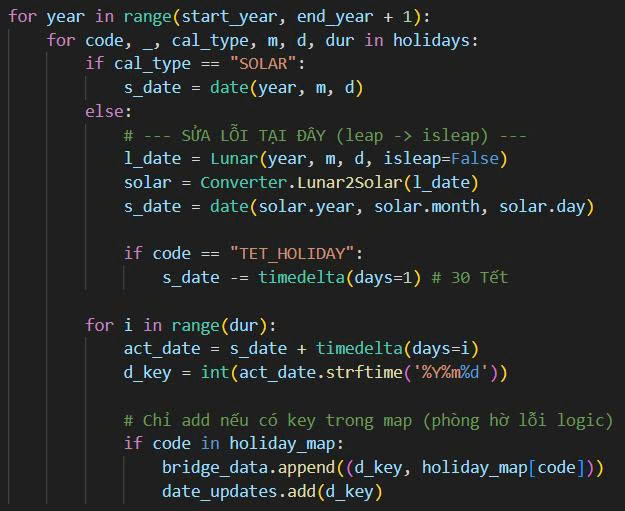
\includegraphics[width=0.7\textwidth]{Images/ETL_07}
    \vspace{6mm}
    \caption{Đoạn mã xử lý chuyển đổi lịch âm sang lịch dương cho ngày lễ}
    \label{fig:etl_07}
\end{figure}

\begin{description}
    \item[C. Cơ chế cầu nối và đồng bộ hóa (Bridge Mechanism)] \hfill \\
    Để giải quyết mối quan hệ nhiều-nhiều (N-N) giữa Ngày và Lễ (một ngày có thể có nhiều lễ, hoặc một lễ kéo dài nhiều ngày), hệ thống sử dụng bảng cầu nối \texttt{bridge\_date\_holiday}:
    \begin{itemize}
        \item \textbf{Ánh xạ khóa ngoại:} Mỗi cặp \texttt{date\_key} (từ \texttt{dim\_date}) và \texttt{holiday\_key} (từ \texttt{dim\_holiday}) được ghi nhận để xác định chính xác sự hiện diện của ngày lễ.
        \item \textbf{Tối ưu hóa hiệu suất truy vấn (De-normalization):} Sau khi nạp dữ liệu vào bảng cầu nối, hệ thống thực hiện một lệnh \texttt{UPDATE} tập hợp lên bảng \texttt{dim\_date}. Toàn bộ các \texttt{date\_key} xuất hiện trong bảng cầu nối sẽ được bật cờ \texttt{is\_holiday = TRUE}.
        \item \textbf{Lợi ích:} Kỹ thuật này giúp các câu lệnh truy vấn lưu lượng giao thông trong ngày lễ sau này chỉ cần lọc theo cờ \texttt{is\_holiday} mà không cần thực hiện phép \texttt{JOIN} phức tạp, giúp tăng tốc độ phản hồi của hệ thống báo cáo.
    \end{itemize}
\end{description}

\begin{figure}[htbp]
    \centering
    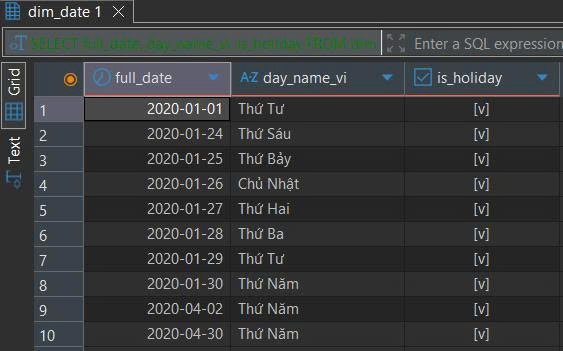
\includegraphics[width=0.7\textwidth]{Images/ETL_08}
    \vspace{6mm}
    \caption{Kết quả cập nhật cờ is\_holiday trong bảng dim\_date}
    \label{fig:etl_08}
\end{figure}

\paragraph{Phân tách và ánh xạ Ca làm việc (Work Shifts)}

Trong phân tích dữ liệu giao thông, việc chỉ sử dụng các mốc giờ thô là không đủ để phản ánh đặc tính vận hành của đô thị. Hệ thống triển khai giải pháp phân tách thời gian dựa trên các "Ca làm việc" (Work Shifts) để hỗ trợ phân tích lưu lượng theo các khung giờ đặc thù như cao điểm sáng, cao điểm chiều và các khung giờ hạn chế giao thông (giờ giới nghiêm cho xe tải).

\begin{description}
    \item[A. Thiết lập danh mục Ca làm việc (dim\_shift)] \hfill \\
    Bảng \texttt{dim\_shift} đóng vai trò định nghĩa các khoảng thời gian vận hành lớn trong một ngày. Dữ liệu này được quản lý thông qua module \texttt{etl/time/etl\_dim\_shift.py} với các quy tắc nghiệp vụ sau:
    \begin{itemize}
        \item \textbf{Phân lớp Ca làm việc:} Hệ thống chia ngày thành 3 phân đoạn chính:
        \begin{itemize}
            \item Ca Sáng (SHIFT\_MORNING): Từ 06:00 đến 14:00 (Phút thứ 360 đến 840). Đây là khung giờ bao gồm cao điểm sáng khi người dân di chuyển đến nơi làm việc.
            \item Ca Chiều (SHIFT\_AFTERNOON): Từ 14:01 đến 22:00 (Phút thứ 841 đến 1320). Khung giờ này bao phủ cao điểm chiều và thời điểm tan sở.
            \item Ca Đêm (SHIFT\_NIGHT): Từ 22:01 đến 05:59 sáng hôm sau (Phút thứ 1321 đến 359). Đây là giai đoạn lưu lượng thấp, chủ yếu phục vụ xe vận tải hạng nặng.
        \end{itemize}
        \item \textbf{Thuộc tính nghiệp vụ (is\_business\_shift):} Mỗi ca được gán một cờ logic để phân biệt giữa khung giờ hành chính và khung giờ nghỉ ngơi, hỗ trợ việc lọc dữ liệu nhanh trong các báo cáo về hiệu suất lao động và kinh tế.
    \end{itemize}

    \item[B. Chi tiết hóa đơn vị thời gian (dim\_time\_of\_day)] \hfill \\
    Để đạt được mức độ chi tiết cao nhất trong phân tích (Granularity), hệ thống không chỉ dừng lại ở mức giờ mà thực hiện "số hóa" đến từng phút trong ngày thông qua bảng \texttt{dim\_time\_of\_day}:
    \begin{itemize}
        \item \textbf{Số hóa 1440 phút:} Module \texttt{etl/time/etl\_dim\_time\_of\_day.py} thực hiện vòng lặp sinh ra chính xác 1440 bản ghi, đại diện cho mỗi phút từ 00:00 đến 23:59. Mỗi bản ghi được định danh bằng một \texttt{time\_key} duy nhất từ 0 đến 1439.
        \item \textbf{Ánh xạ đa chiều (Multi-mapping):} Định dạng HHMM chuyển đổi phút sang dạng số nguyên (ví dụ: 14:05 thành 1405). Liên kết Ca mặc định (\texttt{default\_shift\_key}) sử dụng câu lệnh \texttt{if-elif} để xác định một phút thuộc ca làm việc nào.
        \item \textbf{Định nghĩa Giờ hành chính mặc định:} Hệ thống gán cờ \texttt{is\_business\_hours\_default = TRUE} cho các phút từ 08:00 đến 17:00 (phút 480 đến 1020).
    \end{itemize}

    \item[C. Kỹ thuật nạp dữ liệu tối ưu (Bulk Insert \& Upsert)] \hfill \\
    Xử lý trên RAM bằng cách khởi tạo toàn bộ 1440 bản ghi trong mảng Python (\texttt{data\_buffer}) trước khi đẩy xuống cơ sở dữ liệu. Sử dụng cơ chế \texttt{ON CONFLICT (time\_key) DO UPDATE} để cập nhật các thuộc tính mà không làm thay đổi khóa chính.
\end{description}

\subsubsection{Nhóm chiều Danh mục và Đặc tính (Metadata Dimensions)}

Nhóm chiều Danh mục đóng vai trò là lớp đệm chuẩn hóa, giúp hệ thống đồng nhất các mã dữ liệu thô từ nhiều nguồn khác nhau thành các thông tin có ý nghĩa phân tích thống nhất. Toàn bộ danh mục được quản lý tập trung qua các tệp CSV trong thư mục \texttt{data/}, cho phép cập nhật tham số nghiệp vụ mà không cần can thiệp mã nguồn.

\paragraph{Chuẩn hóa đặc tính phương tiện và hệ số PCU}

Dữ liệu về phương tiện được nạp vào bảng \texttt{dim\_vehicle\_type} thông qua quy trình xử lý tệp \texttt{vehicles.csv}.
\begin{itemize}
    \item \textbf{Hệ số quy đổi xe con (Passenger Car Unit - PCU):} Gán trọng số cụ thể: Xe máy (0.5), Xe con (1.0), Xe tải (2.5). Đây là tham số bắt buộc để đánh giá chính xác mức độ chiếm dụng mặt đường.
    \item \textbf{Tham số vận tốc thiết kế:} Mỗi loại phương tiện được định nghĩa một \texttt{average\_speed\_kmh} làm mốc so sánh (Baseline) cho các mô hình phân tích.
    \item \textbf{Cơ chế nạp dữ liệu an toàn:} Sử dụng \texttt{executemany} kết hợp \texttt{ON CONFLICT (vehicle\_code) DO UPDATE}.
\end{itemize}

\begin{figure}[htbp]
    \centering
    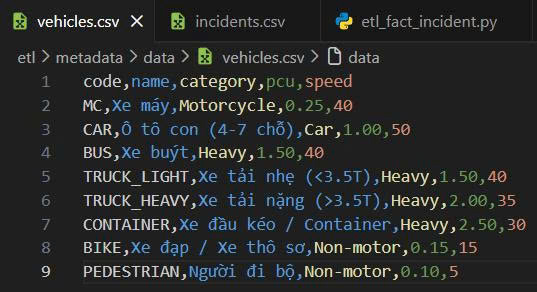
\includegraphics[width=0.7\textwidth]{Images/ETL_09}
    \vspace{6mm}
    \caption{Tệp cấu hình vehicles.csv chứa hệ số PCU và tốc độ thiết kế}
    \label{fig:etl_09}
\end{figure}

\paragraph{Phân loại mức độ nghiêm trọng thời tiết và sự cố}

Chuẩn hóa dữ liệu thô từ API về thang đo thống nhất qua các bảng \texttt{dim\_weather} và \texttt{dim\_incident\_type}.

\begin{description}
    \item[A. Danh mục Điều kiện Thời tiết (Weather Metadata):] \hfill \\
    Dữ liệu được phân loại theo \texttt{severity\_level} từ 1 (Bình thường) đến 4 (Cực đoan). Đi kèm các thuộc tính định tính được mã hóa: \texttt{visibility\_condition} và \texttt{road\_friction\_impact}.
    \item[B. Danh mục Loại hình Sự cố (Incident Metadata):] \hfill \\
    Phân nhóm logic vào các nhóm Tai nạn, Thi công, hoặc Ùn tắc. Đặc biệt tích hợp cột \texttt{color\_hex\_code} (ví dụ: \#FF0000 cho tai nạn) hỗ trợ hiển thị màu sắc biểu tượng trên bản đồ Dashboard một cách tự động.
\end{description}

\begin{figure}[htbp]
    \centering
    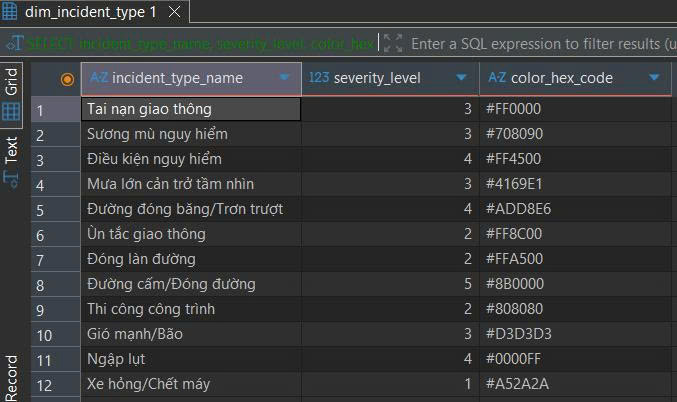
\includegraphics[width=0.9\textwidth]{Images/ETL_10}
    \vspace{6mm}
    \caption{Danh mục sự cố đã chuẩn hóa mã màu trong cơ sở dữ liệu}
    \label{fig:etl_10}
\end{figure}

\subsubsection{Nhóm chiều Hạ tầng Giao thông (Infrastructure Dimensions)}

Chiều hạ tầng giao thông được xác định là thành phần quan trọng nhất, đóng vai trò "xương sống" không gian (Spatial Backbone) của toàn bộ kho dữ liệu. Khác với các chiều dữ liệu định danh thông thường, nhóm này đòi hỏi quy trình xử lý phức tạp dựa trên lý thuyết đồ thị (Graph Theory) và các phép toán hình học không gian để chuyển đổi dữ liệu mạng lưới đường bộ từ OpenStreetMap (OSM) sang định dạng chuẩn của PostGIS. Việc xây dựng nhóm chiều này tuân thủ một trình tự phụ thuộc dữ liệu nghiêm ngặt để đảm bảo tính toàn vẹn tham chiếu: khởi tạo ranh giới hành chính, xây dựng nút giao và tuyến đường, sau đó phân rã thành các phân đoạn nhỏ (Segments).

\paragraph{Trích xuất ranh giới hành chính và Địa điểm (Location ETL)}

Quy trình nạp bảng \texttt{dim\_location} thực hiện định danh và số hóa ranh giới các vùng hành chính, tạo cơ sở cho việc phân tích lưu lượng giao thông theo từng địa phương.

\begin{description}
    \item[A. Kỹ thuật trích xuất dữ liệu không gian từ Overpass API] \hfill \\
    Hệ thống sử dụng thư viện chuyên dụng \texttt{OSMnx} để giao tiếp với API Overpass của OpenStreetMap.
    \begin{itemize}
        \item \textbf{Cơ chế truy vấn:} Gửi các yêu cầu truy vấn hướng đối tượng (Geocode-based requests) thay vì tải dữ liệu thô toàn bộ bản đồ.
        \item \textbf{Phân cấp hành chính:} Trích xuất đa tầng bao gồm Phường/Xã (Ward), Quận/Huyện (District) và Tỉnh/Thành phố (City).
        \item \textbf{Linh hoạt cấu hình:} Danh sách các khu vực trích xuất được tham số hóa để dễ dàng mở rộng phạm vi địa lý.
    \end{itemize}
\end{description}

\begin{figure}[htbp]
    \centering
    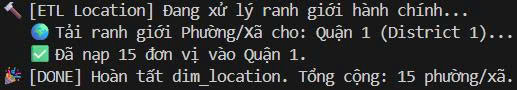
\includegraphics[width=0.7\textwidth]{Images/ETL_11}
    \vspace{6mm}
    \caption{Nhật ký thực thi nạp dữ liệu ranh giới hành chính Quận 1}
    \label{fig:etl_11}
\end{figure}

\begin{description}
    \item[B. Quy trình xử lý hình học (Geometry Processing)] \hfill \\
    Dữ liệu thô sau khi trích xuất cần trải qua các bước biến đổi hình học nghiêm ngặt để tương thích với cơ sở dữ liệu PostGIS:
    \begin{itemize}
        \item \textbf{Chuẩn hóa hệ tọa độ (CRS):} Ép buộc về hệ tọa độ WGS84 (EPSG:4326) để đảm bảo tính đồng nhất khi thực hiện các phép giao cắt không gian sau này.
        \item \textbf{Ép kiểu dữ liệu MULTIPOLYGON:} Lưu trữ dưới dạng \texttt{MULTIPOLYGON} để xử lý các vùng địa giới phức tạp bị chia cắt bởi sông ngòi hoặc hải đảo.
        \item \textbf{Tự động hóa mã hóa (Encoding):} Chuyển đổi đối tượng hình học sang định dạng Hex EWKB (Extended Well-Known Binary) thông qua thư viện \texttt{shapely}.
    \end{itemize}

    \item[C. Ràng buộc dữ liệu và Cơ chế bảo vệ (Data Integrity)] \hfill \\
    Để duy trì tính sạch của kho dữ liệu, hệ thống thiết lập các rào cản kỹ thuật:
    \begin{itemize}
        \item \textbf{Ràng buộc Unique phức hợp:} Thiết lập trên bộ ba cột (ward, district, city) để ngăn chặn trùng lặp bản ghi khi chạy lại quy trình ETL.
        \item \textbf{Chiến lược nạp dữ liệu:} Sử dụng mệnh đề \texttt{ON CONFLICT DO NOTHING} để tối ưu hóa thời gian và giữ nguyên các khóa ngoại đã tham chiếu.
        \item \textbf{Xây dựng mã vị trí (Location Code):} Tự động sinh \texttt{location\_code} chuẩn hóa (ví dụ: PHUONG\_BEN\_NGHE\_QUAN\_1) phục vụ tra cứu nhanh.
    \end{itemize}
\end{description}

\begin{figure}[htbp]
    \centering
    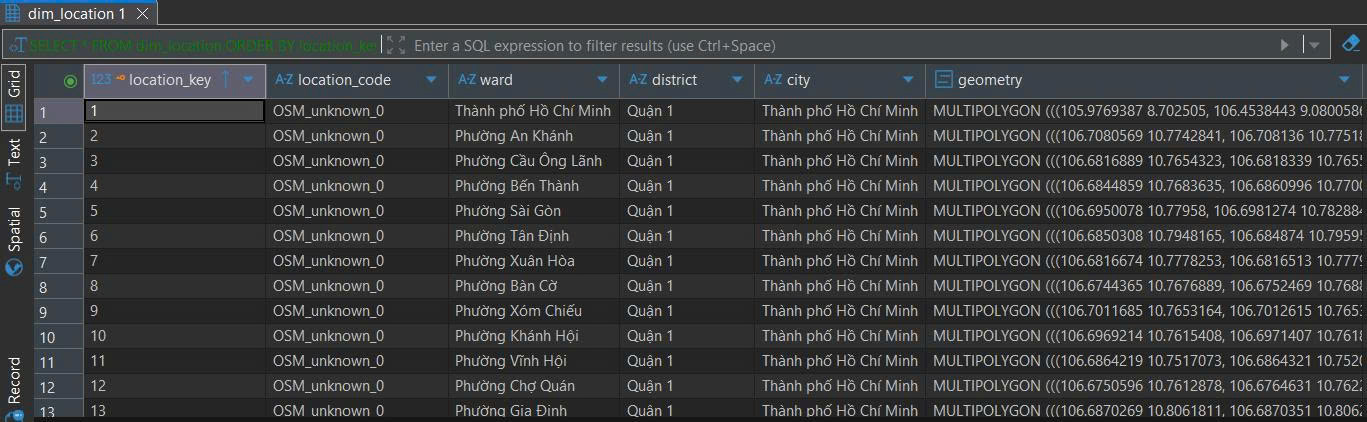
\includegraphics[width=0.9\textwidth]{Images/ETL_12}
    \vspace{6mm}
    \caption{Dữ liệu ranh giới hành chính đã nạp vào bảng dim\_location}
    \label{fig:etl_12}
\end{figure}

\begin{figure}[htbp]
    \centering
    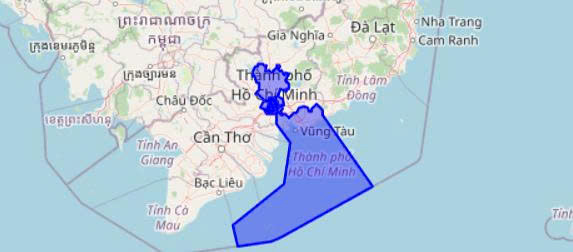
\includegraphics[width=0.5\textwidth]{Images/ETL_13}
    \vspace{6mm}
    \caption{Trực quan hóa đa giác ranh giới TP. Hồ Chí Minh từ PostGIS}
    \label{fig:etl_13}
\end{figure}

\paragraph{ Chuyển đổi mạng lưới đường bộ (Road, Way \& Node ETL)}

Quy trình này biến đổi đồ thị OSM thô thành các thực thể quản lý vật lý và logic.
\begin{itemize}
    \item \textbf{dim\_road (Tuyến đường):} Lưu trữ tên đường logic (ví dụ: Đường Điện Biên Phủ). Một Tuyến đường có thể bao gồm nhiều Đoạn đường vật lý khác nhau.
    \item \textbf{dim\_way (Đoạn đường vật lý):} Lưu trữ các đặc tính kỹ thuật như số làn xe (\texttt{lane\_count}), loại đường (\texttt{way\_type}), và giới hạn tốc độ thiết kế.
    \item \textbf{Số hóa Nút giao (Node ETL):} Toàn bộ các điểm giao cắt, quay đầu được trích xuất thành các bản ghi trong \texttt{dim\_node} dưới dạng một điểm (\texttt{POINT}) với tọa độ chính xác.
\end{itemize}

\paragraph{Phân đoạn và Tính toán hướng đường (Segment ETL)}

Phân đoạn đường (Segment ETL) là bước biến đổi dữ liệu phức tạp nhất, chuyển đổi cấu trúc đồ thị từ các thực thể đường dài (Ways) thành các đơn vị phân tích cơ sở gọi là Segments.

\begin{description}
    \item[A. Quy trình Segment hóa dựa trên cấu trúc đồ thị (Graph-based Segmenting)] \hfill \\
    Chia nhỏ mạng lưới dựa trên các điểm nút (Nodes) để quản lý vi mô các chỉ số giao thông chi tiết đến từng phân đoạn mét đường. Mỗi phân đoạn được cấp một \texttt{segment\_key} duy nhất.

    \item[B. Thuật toán tính toán Azimuth và vai trò trong Map Matching] \hfill \\
    Hướng di chuyển là thông tin sống còn để phân biệt dòng xe trên các đường hai chiều. Hệ thống tính góc hướng (Azimuth) tự động bằng công thức:
    \begin{itemize}
        \item $\Delta Lon = Lon_{to} - Lon_{from}$ 
        \item $\Delta Lat = Lat_{to} - Lat_{from}$ 
        \item $\theta = \operatorname{atan2}(\Delta Lon, \Delta Lat)$ 
    \end{itemize}
    Kết quả được chuẩn hóa về khoảng $[0^\circ, 360^\circ]$ để thực hiện kỹ thuật Map Matching, giúp đối khớp chính xác dữ liệu tốc độ thời gian thực từ TomTom API vào đúng hướng di chuyển tương ứng.

    \item[C. Chiến lược đa dạng hóa dữ liệu hình học (Dual-Geometry Strategy)] \hfill \\
    Mỗi Segment lưu trữ đồng thời hai loại dữ liệu không gian để tối ưu hóa hiển thị và hiệu năng xử lý:
    \begin{itemize}
        \item \textbf{geometry\_linestring (Chuỗi đường):} Lưu trữ tọa độ tạo nên hình dáng uốn lượn thực tế của đoạn đường, dùng để vẽ bản đồ nhiệt hoặc lộ trình.
        \item \textbf{geometry\_center (Điểm trung tâm):} Tính toán điểm trọng tâm (\texttt{Centroid}) của đoạn đường để tăng tốc các phép toán tìm kiếm lân cận hoặc giao cắt hành chính (Spatial Join).
    \end{itemize}
\end{description}

\begin{figure}[htbp]
    \centering
    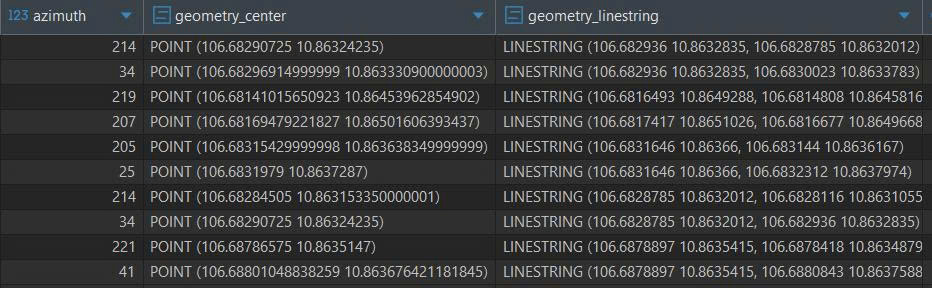
\includegraphics[width=1.0\textwidth]{Images/ETL_14}
    \vspace{6mm}
    \caption{Dữ liệu góc Azimuth và hình học đa tầng trong bảng dim\_segment}
    \label{fig:etl_14}
\end{figure}
\paragraph{Làm giàu dữ liệu bằng phép giao không gian (Spatial Enrichment)}

Sau khi hoàn tất việc nạp dữ liệu vào các bảng hạ tầng độc lập, kho dữ liệu vẫn tồn tại một khoảng cách giữa thực thể kỹ thuật (các phân đoạn đường OSM) và thực thể quản lý hành chính (Phường, Quận). Để giải quyết bài toán này, hệ thống triển khai bước "Enrichment" (Làm giàu dữ liệu) thông qua module \texttt{etl/infrastructure/etl\_enrichment.py}. Đây là quy trình hậu xử lý quan trọng nhằm thiết lập mối quan hệ logic giữa Hạ tầng và Hành chính một cách hoàn toàn tự động dựa trên tọa độ địa lý.

\begin{description}
    \item[A. Cơ chế Spatial Join thông qua hàm hình học PostGIS] \hfill \\
    Thay vì yêu cầu người dùng nhập liệu thủ công hoặc dựa vào các bảng tra cứu tĩnh dễ sai sót, hệ thống tận dụng sức mạnh xử lý không gian trực tiếp bên trong Database:
    \begin{itemize}
        \item \textbf{Thuật toán kiểm tra điểm trong đa giác (Point-in-Polygon):} Hệ thống thực thi các câu lệnh SQL sử dụng hàm \texttt{ST\_Contains} (hoặc \texttt{ST\_Within}) để đối chiếu hình học.
        \item \textbf{Quy trình xác định:} Quét qua toàn bộ các Segment có cột \texttt{location\_key} đang trống và xác định xem điểm trung tâm (\texttt{geometry\_center}) của đoạn đường đó nằm gọn trong đa giác ranh giới (\texttt{geometry}) nào của bảng \texttt{dim\_location}.
        \item \textbf{Tại sao sử dụng Điểm trung tâm (Geometry Center):} Một đoạn đường (\texttt{LineString}) có thể đi ngang qua ranh giới giữa hai phường, gây ra lỗi đa trùng lặp nếu thực hiện phép giao cắt toàn phần. Việc sử dụng điểm trung tâm giúp đảm bảo mỗi đoạn đường chỉ được gán duy nhất cho một đơn vị hành chính.
    \end{itemize}
\end{description}

\begin{figure}[htbp]
    \centering
    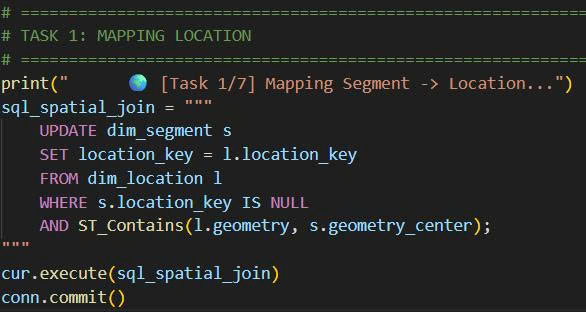
\includegraphics[width=0.8\textwidth]{Images/ETL_15}
    \vspace{6mm}
    \caption{Câu lệnh SQL thực hiện phép giao không gian để cập nhật location\_key}
    \label{fig:etl_15}
\end{figure}

\begin{description}
    \item[B. Tự động hóa cập nhật và tính nhất quán dữ liệu] \hfill \\
    Kết quả của phép giao không gian này là cột \texttt{location\_key} trong bảng \texttt{dim\_segment} được cập nhật giá trị tham chiếu chính xác đến bảng \texttt{dim\_location}. Nhờ có bước Enrichment này, mọi bản ghi Fact sau khi được gắn vào \texttt{segment\_key} sẽ nghiễm nhiên sở hữu thông tin hành chính thông qua mối quan hệ bắc cầu, hỗ trợ các báo cáo tổng hợp như "Tính toán tốc độ trung bình của toàn bộ các đoạn đường thuộc Quận 1" mà không cần can thiệp mã nguồn ETL.

    \item[C. Tối ưu hóa hiệu năng xử lý không gian (Spatial Indexing)] \hfill \\
    Do số lượng Segment có thể lên đến hàng chục nghìn bản ghi, hệ thống sử dụng \textbf{GIST Index} trên cột điểm trung tâm và chỉ mục không gian trên cột đa giác ranh giới của \texttt{dim\_location}. Điều này cho phép Database thực hiện phép giao không gian với độ phức tạp logarit thay vì quét toàn bộ bảng.
\end{description}

\subsection{QUY TRÌNH NẠP DỮ LIỆU SỰ KIỆN (FACT ETL PIPELINE)}

Quy trình nạp dữ liệu sự kiện (Fact ETL) là giai đoạn quan trọng nhất trong vận hành hàng ngày của hệ thống. Khác với dữ liệu Dimension mang tính chất tĩnh, dữ liệu Fact được thiết kế để thu thập các biến động không ngừng của mạng lưới giao thông theo thời gian thực (Real-time). Quy trình này thực hiện việc kết hợp dữ liệu từ các nguồn API quốc tế với dữ liệu quan trắc trực tiếp từ mô hình AI để tạo ra cái nhìn toàn diện về thực trạng giao thông.

\subsubsection{Tầng Dịch vụ thu thập dữ liệu (Data Service Layer)}

Để đảm bảo tính module hóa và dễ bảo trì, hệ thống tách biệt logic giao tiếp với các nhà cung cấp dữ liệu bên ngoài thành một tầng dịch vụ riêng biệt (\texttt{Service Layer}). Tầng này chịu trách nhiệm đóng gói các yêu cầu API, xử lý xác thực và chuẩn hóa dữ liệu thô (JSON) trước khi đưa vào các pipeline xử lý chính.

\begin{description}
    \item[a. Dịch vụ dữ liệu giao thông (TomTom Service)] \hfill \\
    Module \texttt{modules/tomtom\_service.py} là thành phần chịu trách nhiệm tương tác với TomTom:
    \begin{itemize}
        \item \textbf{Trích xuất dữ liệu lưu lượng (Traffic Flow):} Sử dụng endpoint \texttt{flowSegmentData} để truy vấn tốc độ di chuyển thực tế (\texttt{currentSpeed}) và tốc độ tự do (\texttt{freeFlowSpeed}) tại một tọa độ cụ thể.
        \item \textbf{Trích xuất dữ liệu sự cố (Traffic Incidents):} Sử dụng cơ chế quét theo vùng (Bounding Box) để lấy loại sự cố, tọa độ hình học, độ trễ và mô tả chi tiết sự việc.
    \end{itemize}
\end{description}

\begin{figure}[htbp]
    \centering
    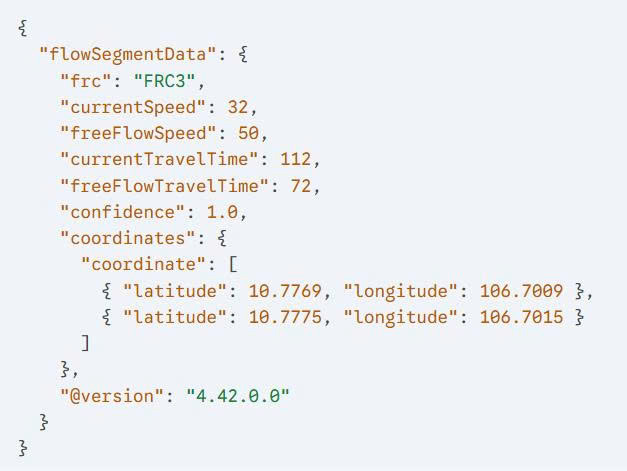
\includegraphics[width=0.6\textwidth]{Images/ETL_16}
    \vspace{6mm}
    \caption{Cấu trúc dữ liệu JSON trả về từ TomTom Traffic API}
    \label{fig:etl_16}
\end{figure}

\begin{description}
    \item[b. Dịch vụ dữ liệu khí tượng (Weather Service)] \hfill \\
    Dữ liệu thời tiết được cung cấp bởi module \texttt{modules/weather\_service.py} thông qua OpenWeatherMap API. Hệ thống thực hiện truy vấn theo tọa độ chính xác của từng đoạn đường (\textit{lat, lon}) để đảm bảo tính cục bộ, trả về các thông số: mã thời tiết (Weather ID), nhiệt độ, độ ẩm, tầm nhìn (\textit{visibility}) và lượng mưa.
\end{description}

\subsubsection{Tích hợp Thị giác máy tính trong quy trình ETL (AI Integration)}

Một điểm sáng tạo và đột phá của đồ án là việc tích hợp trực tiếp mô hình học sâu (Deep Learning) vào luồng xử lý dữ liệu Fact để thu thập số lượng phương tiện thực tế, thay vì chỉ dựa vào dữ liệu ước tính từ API.

\paragraph{ Kiến trúc bộ đếm phương tiện dựa trên YOLOv8}

Dự án triển khai module \texttt{modules/ai\_counter.py} để thu thập dữ liệu "ground truth" từ các nguồn camera giao thông trực tuyến.



\begin{description}
    \item[A. Lựa chọn mô hình YOLOv8x (Extra Large) cho độ chính xác tối ưu] \hfill \\
    Hệ thống sử dụng kiến trúc \textbf{YOLOv8} phiên bản "x" (Extra Large) cho độ chính xác cao nhất. Việc lựa chọn mô hình này là cần thiết để giải quyết bài toán mật độ phương tiện cực cao tại các nút giao thông TP.HCM, giúp nhận diện chính xác các đối tượng nhỏ như xe máy trong điều kiện bị che khuất (Occlusion).
\end{description}

\begin{figure}[htbp]
    \centering
    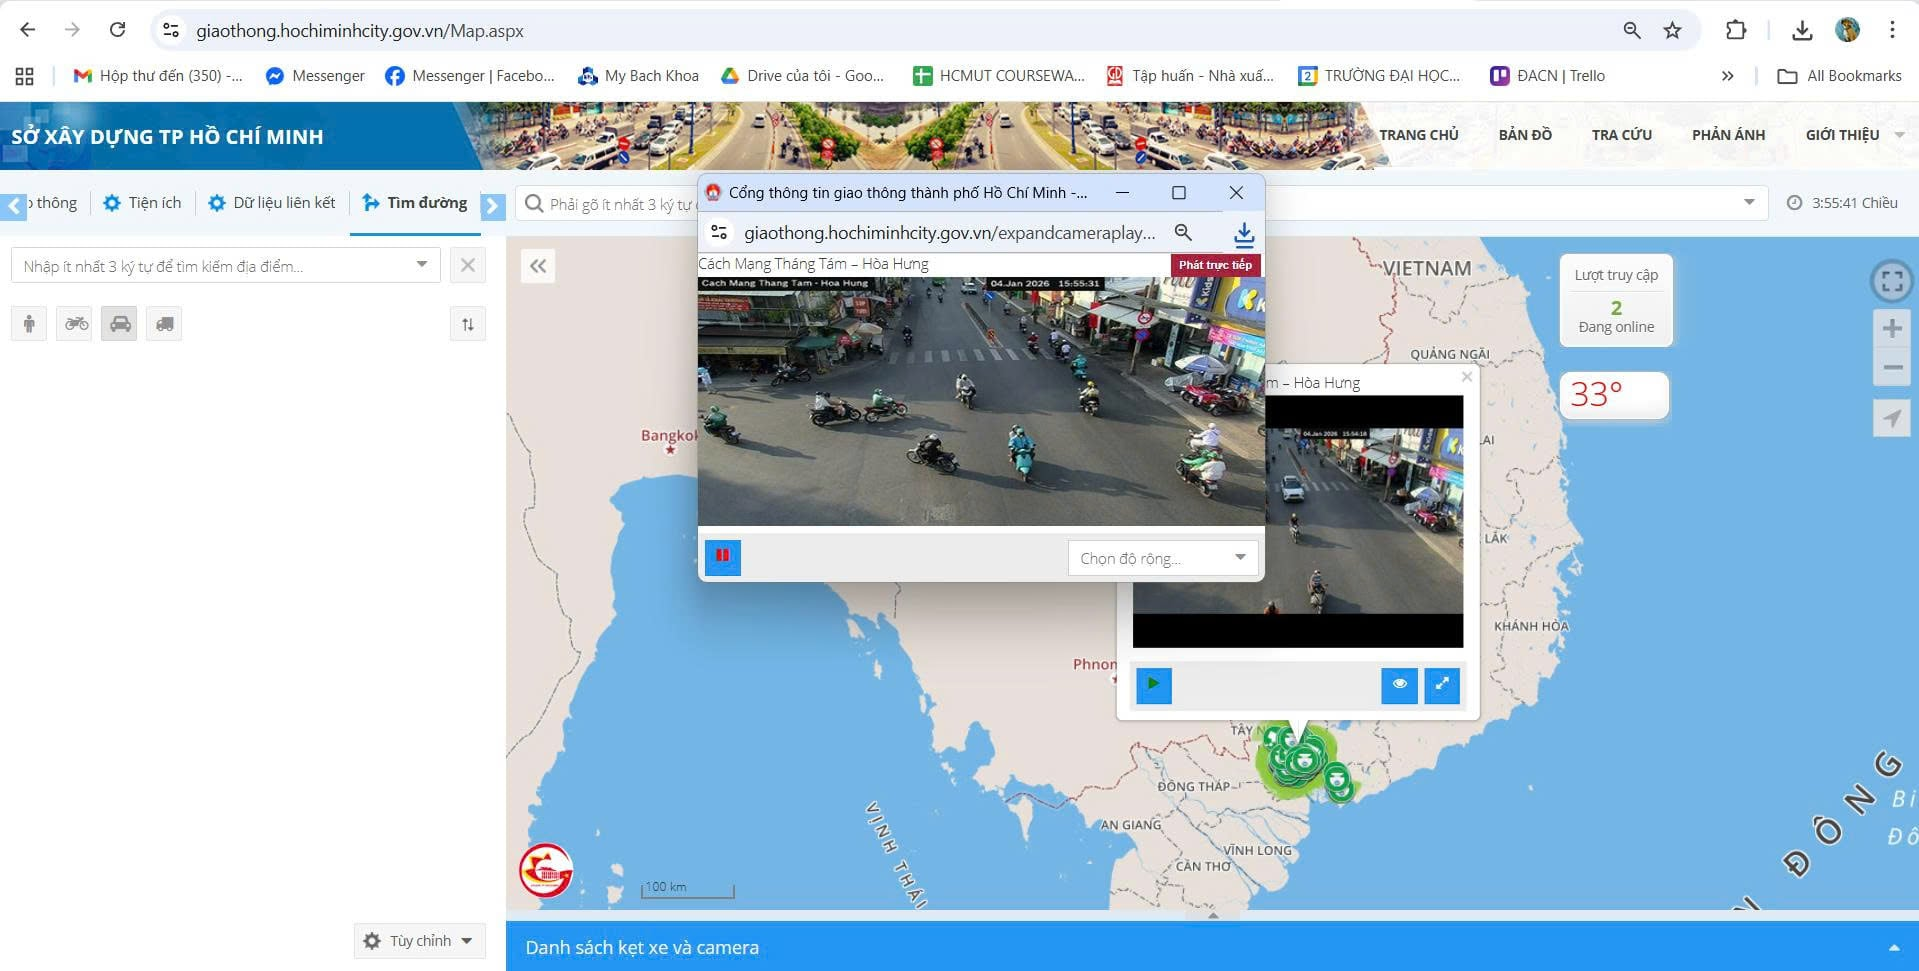
\includegraphics[width=1.0\textwidth]{Images/ETL_17a}
    \vspace{6mm}
    \caption{Trang web lấy hình ảnh camera tại Đường Cách Mạng Tháng Tám - Hòa Hưng}
    \label{fig:etl_17a}
\end{figure}

\begin{figure}[htbp]
    \centering
    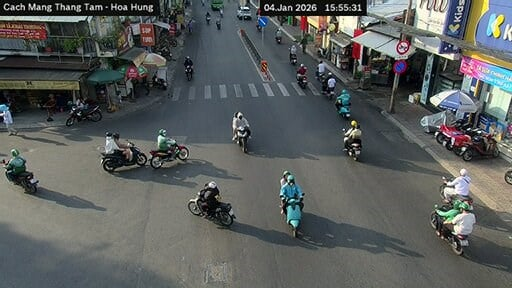
\includegraphics[width=1.0\textwidth]{Images/ETL_17b}
    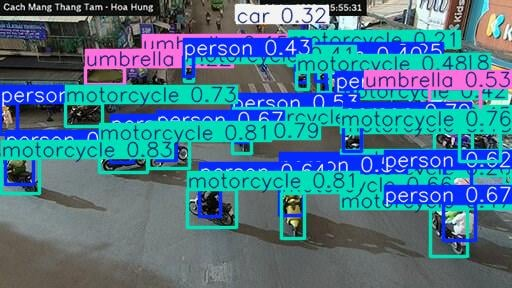
\includegraphics[width=1.0\textwidth]{Images/ETL_17}
    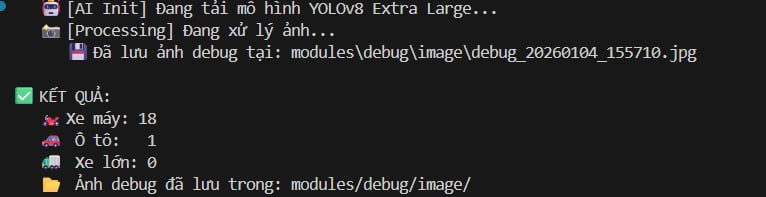
\includegraphics[width=1.0\textwidth]{Images/ETL_17c}
    \vspace{6mm}
    \caption{Kết quả nhận diện và phân lớp phương tiện thời gian thực bằng YOLOv8x}
    \label{fig:etl_17}
\end{figure}


\newpage
\begin{description}
    \item[B. Phân lớp đối tượng và Cơ chế lọc lớp (Class Filtering)] \hfill \\
    Hệ thống cấu hình \texttt{self.target\_classes = [2, 3, 5, 7]} để chỉ tập trung vào mảng giao thông:
    \begin{itemize}
        \item \textbf{Class 2 (Car):} Ánh xạ vào nhóm xe ô tô con.
        \item \textbf{Class 3 (Motorcycle):} Nhóm xe máy chiếm tỷ trọng lớn nhất tại Việt Nam.
        \item \textbf{Class 5 (Bus) và Class 7 (Truck):} Được gộp vào nhóm xe tải/xe hạng nặng (\texttt{heavy\_vehicle\_count}).
    \end{itemize}
    Các đối tượng nhiễu như người đi bộ, động vật hay biển báo đều bị bỏ qua ngay tại tầng xử lý AI.
\end{description}

\begin{figure}[htbp]
    \centering
    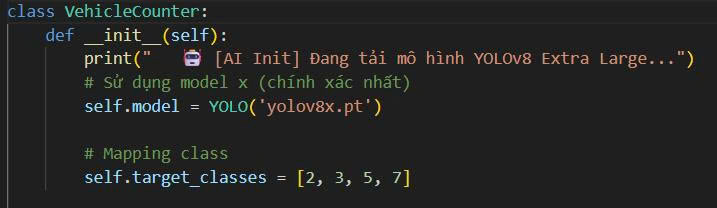
\includegraphics[width=0.8\textwidth]{Images/ETL_18}
    \vspace{6mm}
    \caption{Khởi tạo mô hình YOLOv8 và cấu hình danh mục đối tượng mục tiêu}
    \label{fig:etl_18}
\end{figure}
\paragraph{Quy trình chuẩn hóa dữ liệu AI và Tính toán lưu lượng quy đổi (PCU)}

Sau khi mô hình YOLOv8 hoàn tất việc phát hiện và gán nhãn các đối tượng trong khung hình, dữ liệu vẫn ở dạng danh sách các "Bounding Boxes" rời rạc. Quy trình ETL tiếp tục thực hiện bước chuẩn hóa dữ liệu và áp dụng các công thức nghiệp vụ để biến đổi chúng thành các chỉ số lưu lượng mang tính kỹ thuật.

\begin{description}
    \item[A. Cơ chế tổng hợp và Phân nhóm phương tiện (Aggregation Logic)] \hfill \\
    Hệ thống triển khai một hàm băm (Mapping Function) để chuyển đổi từ 80 lớp của tập dữ liệu COCO về 4 nhóm thực thể chính phù hợp với hạ tầng giao thông Việt Nam:
    \begin{itemize}
        \item \textbf{Nhóm xe máy (motorcycle\_count):} Được trích xuất trực tiếp từ class ID 3. Đây là nhóm đối tượng có kích thước nhỏ và mật độ dày đặc nhất, đòi hỏi độ chính xác cao trong nhận diện.
        \item \textbf{Nhóm xe con (car\_count):} Trích xuất từ class ID 2.
        \item \textbf{Nhóm xe hạng nặng (heavy\_vehicle\_count):} Hệ thống thực hiện phép hợp (Union) các đối tượng thuộc class 5 (Bus) và class 7 (Truck). Việc gộp nhóm này giúp đơn giản hóa bài toán tính toán tải trọng lên mặt đường.
        \item \textbf{Nhóm phương tiện khác (other\_count):} Bao gồm các lớp như xe đạp, xe lôi hoặc các phương tiện không xác định khác để đảm bảo không bỏ sót bất kỳ thực thể nào đang chiếm dụng không gian đường bộ.
    \end{itemize}

    \item[B. Thuật toán tính toán lưu lượng quy đổi (PCU Calculation)] \hfill \\
    Để đánh giá chính xác mức độ tắc nghẽn, hệ thống quy đổi số lượng xe về đơn vị xe con tiêu chuẩn (Passenger Car Unit - PCU). Công thức được cài đặt trực tiếp trong module \texttt{ai\_counter.py} dựa trên các hệ số thực nghiệm:
    \begin{equation}
        Total\_PCU = N_{moto} \times 0.25 + N_{car} \times 1.0 + N_{heavy} \times 2.0 + N_{other} \times 1.0
    \end{equation}
    Việc sử dụng hệ số 0.25 cho xe máy phản ánh thực tế rằng diện tích chiếm dụng động của một xe máy chỉ bằng 1/4 so với một xe ô tô con tiêu chuẩn. Chỉ số \texttt{total\_pcu} là dữ liệu đầu vào quan trọng nhất để tính toán mật độ dòng chảy và khả năng thông hành của đoạn đường.
\end{description}

\begin{figure}[htbp]
    \centering
    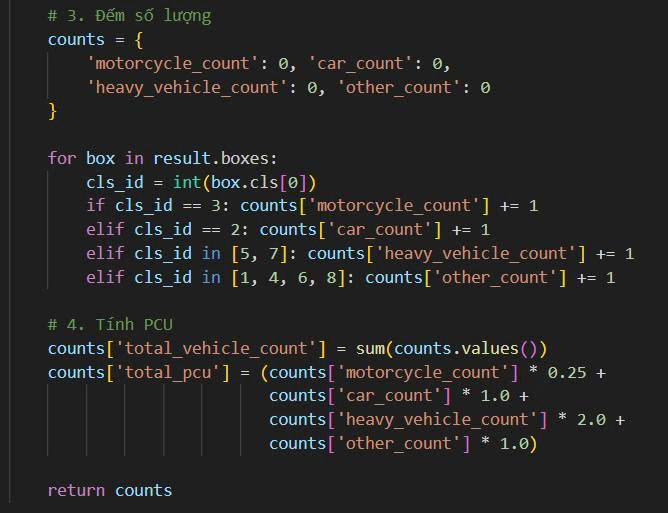
\includegraphics[width=0.8\textwidth]{Images/ETL_19}
    \vspace{6mm}
    \caption{Đoạn mã triển khai logic đếm đối tượng và tính toán PCU từ kết quả AI}
    \label{fig:etl_19}
\end{figure}

\subsubsection{Xác định chỉ số LOS (Level of Service) và Mức độ ùn tắc}

Từ dữ liệu AI và vận tốc thu thập được, hệ thống tiến hành phân loại chất lượng dòng lưu lượng thông qua chỉ số LOS (A-F) ngay trong module \texttt{etl\_fact\_traffic.py}:

\begin{itemize}
    \item \textbf{Công thức tính Congestion Level:} Hệ thống so sánh tốc độ thực tế (\texttt{current\_speed}) với tốc độ tự do (\texttt{free\_flow\_speed}) để tính toán tỷ lệ phần trăm ùn tắc.
    \item \textbf{Phân cấp LOS:}
    \begin{itemize}
        \item \textbf{LOS A/B:} Dòng xe lưu thông tự do, tốc độ thực tế gần bằng tốc độ thiết kế (Congestion $<$ 15\%).
        \item \textbf{LOS C/D:} Dòng xe bắt đầu bị ảnh hưởng, người lái khó thay đổi làn đường (Congestion 15\% - 45\%).
        \item \textbf{LOS E/F:} Dòng xe bị ùn tắc nghiêm trọng hoặc đứng im, tốc độ giảm sâu (Congestion $>$ 45\%).
    \end{itemize}
    \item \textbf{Ghi nhận dữ liệu:} Toàn bộ các chỉ số này được đóng gói thành một bản ghi và đẩy vào phân vùng tương ứng của bảng \texttt{fact\_traffic\_flow}.
\end{itemize}

\begin{figure}[htbp]
    \centering
    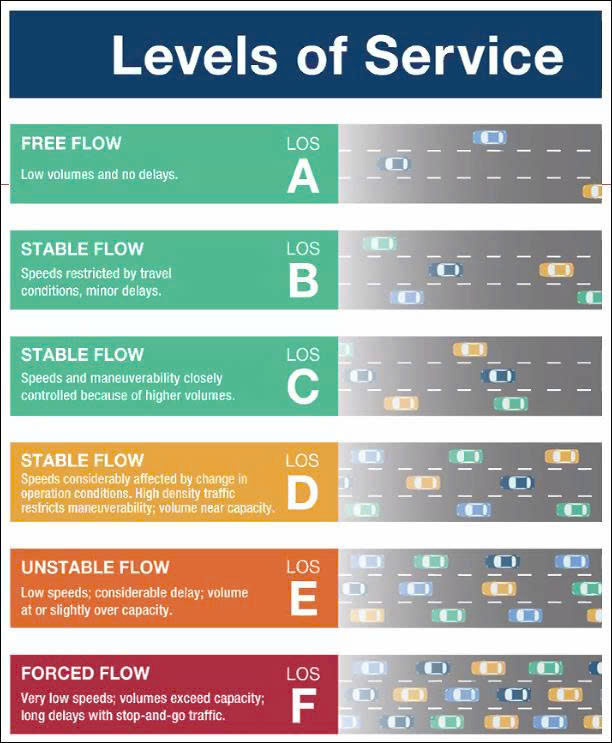
\includegraphics[width=0.6\textwidth]{Images/ETL_20}
    \vspace{6mm}
    \caption{Mô tả các cấp độ phục vụ (LOS) trong kỹ thuật giao thông}
    \label{fig:etl_20}
\end{figure}

\subsubsection{ Quy trình nạp dữ liệu Fact Traffic Flow và Fact Incident}

Các bảng Fact là trái tim của Star Schema, lưu trữ các chỉ số định lượng về trạng thái mạng lưới giao thông. Quy trình nạp dữ liệu vào bảng Fact yêu cầu sự kết hợp phức tạp giữa các kỹ thuật đối khớp không gian (Spatial Matching) và logic nghiệp vụ để đảm bảo tính nhất quán giữa dữ liệu động và hạ tầng tĩnh.

\paragraph{ Quy trình nạp dữ liệu Lưu lượng Giao thông (Fact Traffic Flow ETL)}

Đây là quy trình quan trọng nhất trong hệ thống, thực hiện nhiệm vụ tổng hợp và đồng bộ hóa dữ liệu từ ba nguồn khác nhau: Trí tuệ nhân tạo (AI), API Giao thông (TomTom) và API Thời tiết (OpenWeatherMap) thành một bản ghi thông tin duy nhất đại diện cho trạng thái của một phân đoạn đường tại một thời điểm cụ thể.

\begin{description}
    \item[A. Cơ chế Hợp nhất dữ liệu đa nguồn (Multi-source Data Fusion)] \hfill \\
    Hệ thống tập trung vào các vị trí chiến lược được định nghĩa trong cấu hình \texttt{CAMERA\_MAPPING}. Pipeline thực hiện quét qua danh sách các \texttt{segment\_key} có gắn camera giám sát. Với mỗi Segment, hệ thống đóng vai trò như một bộ não trung tâm, kích hoạt đồng thời hai luồng thu thập dữ liệu:
    \begin{itemize}
        \item \textbf{Luồng quan trắc mật độ (AI Stream):} Gọi module \texttt{ai\_counter.py} để phân tích ảnh camera, trả về số lượng chi tiết từng loại xe và tổng lưu lượng quy đổi PCU.
        \item \textbf{Luồng quan trắc vận tốc (API Stream):} Gọi \texttt{tomtom\_service.py} để lấy tốc độ di chuyển thực tế và tốc độ tự do tại đúng tọa độ của phân đoạn đó.
    \end{itemize}
    Việc kết hợp giữa "Mật độ" (từ AI) và "Vận tốc" (từ API) cho phép hệ thống xây dựng được biểu đồ quan hệ cơ bản của dòng giao thông (Fundamental Diagram of Traffic Flow).

    \item[B. Quy trình xác định khóa tham chiếu và Liên kết ngữ cảnh (Key Mapping)] \hfill \\
    Để dữ liệu Fact có thể liên kết được với các bảng Dimension, hệ thống thực hiện ánh xạ khóa nghiêm ngặt:
    \begin{itemize}
        \item \textbf{Khóa thời gian (Temporal Keys):} Thời gian thực thi được băm nhỏ thành \texttt{time\_key} (phút trong ngày) và \texttt{date\_key} (YYYYMMDD) để thực hiện các phép Join cực nhanh bằng kiểu dữ liệu Integer.
        \item \textbf{Khóa ngữ cảnh thời tiết (Weather Key):} Tại mỗi vị trí camera, hệ thống gọi dịch vụ thời tiết để ghi nhận điều kiện khí tượng tức thời. Mã thời tiết trả về được ánh xạ thành \texttt{weather\_key}, hỗ trợ phân tích tương quan giữa thời tiết và lưu lượng xe.
    \end{itemize}
\end{description}

\begin{figure}[htbp]
    \centering
    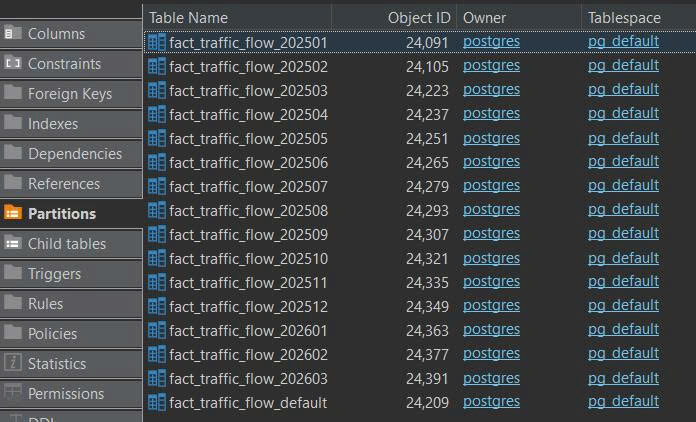
\includegraphics[width=0.8\textwidth]{Images/ETL_21}
    \vspace{6mm}
    \caption{Cấu trúc các phân vùng bảng Fact theo tháng trong PostgreSQL}
    \label{fig:etl_21}
\end{figure}

\begin{description}
    \item[C. Tính toán chỉ số hiệu suất và Phân cấp LOS (Performance Metrics)] \hfill \\
    Sau khi hợp nhất dữ liệu, hệ thống tính toán \texttt{congestion\_level} dựa trên tỷ lệ giữa tốc độ hiện tại và tốc độ tự do. Hệ thống áp dụng bộ quy tắc phân loại LOS từ A đến F để đánh giá chất lượng dịch vụ. Toàn bộ bản ghi được nạp theo lô (Batch Load) vào Database thông qua hàm \texttt{executemany} để tối ưu hóa hiệu năng ghi.
\end{description}

\begin{figure}[htbp]
    \centering
    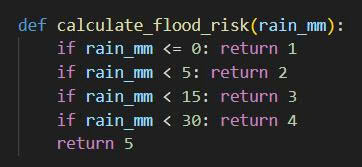
\includegraphics[width=0.8\textwidth]{Images/ETL_22}
    \vspace{6mm}
    \caption{Hàm xử lý logic tính toán chỉ số rủi ro ngập lụt}
    \label{fig:etl_22}
\end{figure}
\paragraph{ Quy trình nạp dữ liệu Sự cố Giao thông (Fact Incident ETL)}

Bảng \texttt{fact\_incident} đóng vai trò lưu trữ các sự kiện bất thường gây ảnh hưởng đến năng lực thông hành của mạng lưới đường bộ như tai nạn, thi công, hoặc thời tiết cực đoan. Quy trình ETL cho bảng này, được triển khai trong module \texttt{etl/fact/etl\_fact\_incident.py}, giải quyết bài toán thách thức về đối khớp một điểm tọa độ sự cố tự do vào một đoạn đường quản lý cụ thể (Point-to-Segment Mapping).

\begin{description}
    \item[A. Thuật toán Tìm kiếm phân đoạn gần nhất (Spatial Lookup) dựa trên Haversine] \hfill \\
    Dữ liệu sự cố từ TomTom API trả về dưới dạng tọa độ kinh/vĩ độ (\texttt{Point}). Tuy nhiên, để dữ liệu này có giá trị phân tích, sự cố phải được gắn (\texttt{Link}) chính xác với một \texttt{segment\_key} trong kho dữ liệu.
    \begin{itemize}
        \item \textbf{Tính toán khoảng cách địa cầu:} Do PostGIS thực hiện các phép tính trên mặt cầu, hệ thống triển khai hàm \texttt{calculate\_distance\_haversine} để đo khoảng cách chính xác theo đường chim bay giữa vị trí sự cố và điểm trung tâm (\texttt{geometry\_center}) của từng đoạn đường.
        \item \textbf{Công thức áp dụng:} Hệ thống sử dụng bán kính Trái đất $R = 6,371,000$ mét và các phép tính lượng giác để xác định khoảng cách chính xác đến từng mét.
        \item \textbf{Chiến lược lựa chọn đối tượng:} Hệ thống thực hiện quét trong bán kính lân cận (dưới 50m - 100m) để tìm phân đoạn phù hợp nhất. Nếu sự cố nằm quá xa các đoạn đường đã số hóa (vượt ngưỡng sai số GPS), hệ thống sẽ tự động ghi nhận vào log và bỏ qua (\texttt{skipped\_count}) để đảm bảo tính sạch của dữ liệu.
    \end{itemize}

    \item[B. Cơ chế Ánh xạ loại sự cố (Incident Type Mapping)] \hfill \\
    TomTom sử dụng hệ thống mã số riêng để định danh loại sự kiện. Hệ thống ETL thực hiện bước chuẩn hóa dữ liệu thông qua từ điển ánh xạ \texttt{TOMTOM\_INCIDENT\_MAP}:
    \begin{itemize}
        \item \textbf{Đồng nhất hóa danh mục:} Mọi sự cố từ API được chuyển đổi sang các mã chuẩn như \texttt{ACCIDENT}, \texttt{ROAD\_WORK}, \texttt{FLOOD}... đã được định nghĩa trong bảng \texttt{dim\_incident\_type}.
        \item \textbf{Tích hợp bối cảnh khí tượng:} Ngay khi một sự cố được ghi nhận, hệ thống đồng thời gọi \texttt{get\_weather\_by\_coords} để lấy thông tin thời tiết tại thời điểm đó, hỗ trợ phân tích các yếu tố tác động ngoại cảnh.
    \end{itemize}

    \item[C. Cấu trúc nạp dữ liệu và Quản lý dòng thời gian (Loading \& Timeline)] \hfill \\
    Dữ liệu sự cố được nạp với đầy đủ các thuộc tính: ghi nhận thời gian tồn tại (\texttt{start\_time} và \texttt{expected\_end\_time}) để tính toán tổng thời gian ảnh hưởng; ghi nhận chỉ số tác động (\texttt{delay\_seconds} và \texttt{length\_meters}). Hệ thống sử dụng kỹ thuật \texttt{Batch Insert} để nạp một lần duy nhất vào PostgreSQL, giúp giảm độ trễ và tránh tình trạng khóa bảng.
\end{description}

\begin{figure}[htbp]
    \centering
    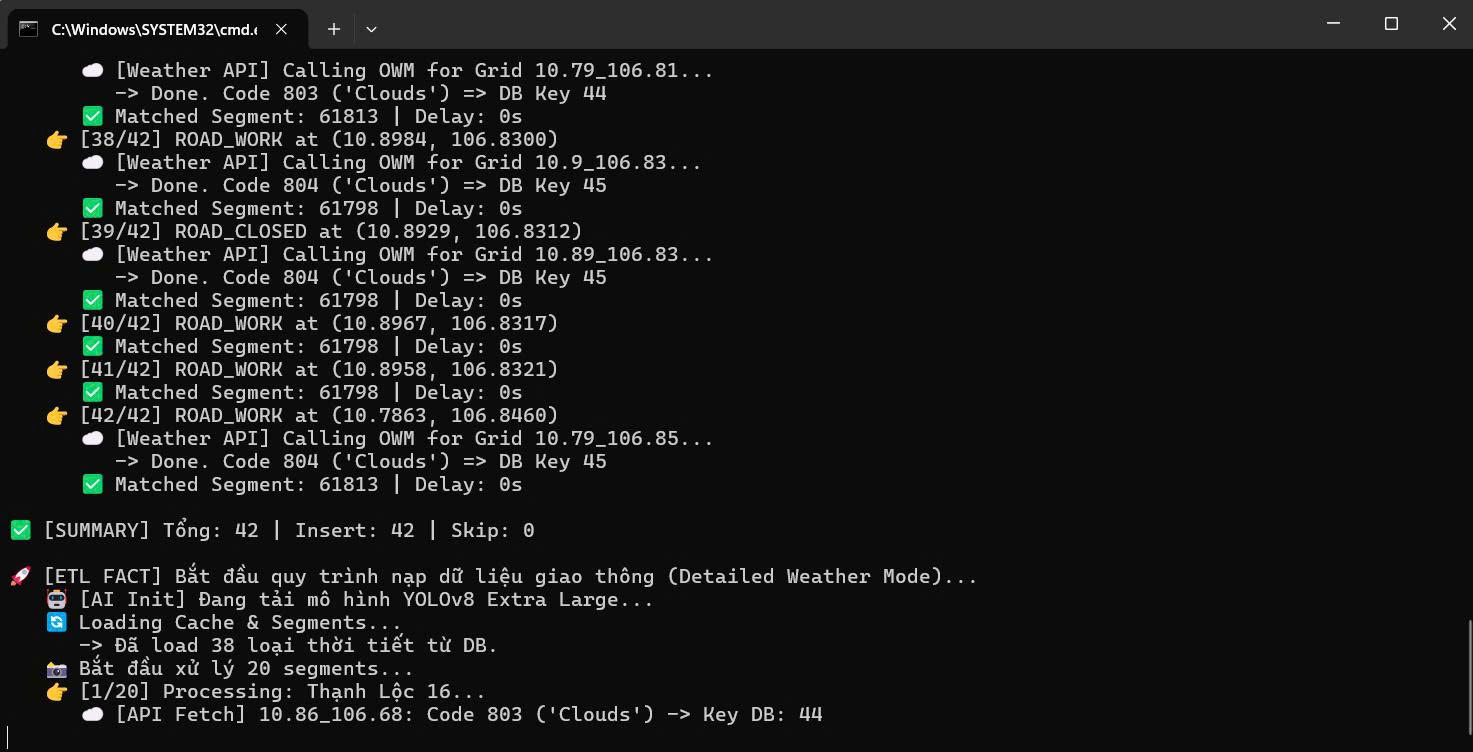
\includegraphics[width=0.8\textwidth]{Images/ETL_23}
    \vspace{6mm}
    \caption{Nhật ký nạp dữ liệu sự cố và kết quả đối khớp không gian thành công}
    \label{fig:etl_23}
\end{figure}

\paragraph{Chiến lược Quản trị Phân vùng và Hiệu năng (Partitioning \& Performance)}

Với tần suất nạp dữ liệu 15 phút/lần, các bảng Fact sẽ nhanh chóng tích lũy hàng triệu bản ghi. Để đảm bảo hệ thống không bị suy giảm hiệu năng, dự án triển khai các kỹ thuật quản trị dữ liệu quy mô lớn ngay từ tầng vật lý.

\begin{description}
    \item[A. Kỹ thuật Phân vùng dữ liệu theo dải thời gian (Range Partitioning)] \hfill \\
    Áp dụng tính năng \texttt{Declarative Partitioning} cho bảng \texttt{fact\_traffic\_flow}. Dữ liệu được phân tán vào các bảng con dựa trên giá trị của \texttt{date\_key} theo từng tháng (ví dụ: \texttt{fact\_traffic\_flow\_202501}). Việc này giúp tránh hiện tượng "Bloat" dữ liệu, giảm chi phí bảo trì chỉ mục và cho phép thực hiện cơ chế \texttt{Partition Pruning} khi truy vấn, giúp tăng tốc độ phản hồi đáng kể.

    \item[B. Tối ưu hóa hệ thống chỉ mục đa tầng (Multi-level Indexing)] \hfill \\
    Thiết lập chỉ mục \texttt{B-Tree} trên các khóa ngoại (\texttt{segment\_key}, \texttt{time\_key}, \texttt{date\_key}) để tối ưu các phép toán \texttt{JOIN}. Đặc biệt, chỉ mục không gian \texttt{GIST} được đánh trên cột \texttt{geometry} của bảng \texttt{fact\_incident}, cho phép thực hiện các truy vấn phức tạp như tìm kiếm sự cố trong bán kính người dùng hoặc vẽ bản đồ nhiệt (\texttt{Heatmap}) với độ phức tạp logarit.

    \item[C. Lợi ích tổng thể về vận hành] \hfill \\
    Đảm bảo thời gian chạy của mỗi batch ETL luôn ổn định dưới 2 phút. Đồng thời, dễ dàng thực hiện việc lưu trữ (\texttt{Archiving}) hoặc xóa dữ liệu cũ bằng cách ngắt kết nối (\texttt{Detach}) một phân vùng tháng mà không làm gián đoạn hệ thống đang chạy.
\end{description}

\begin{figure}[htbp]
    \centering
    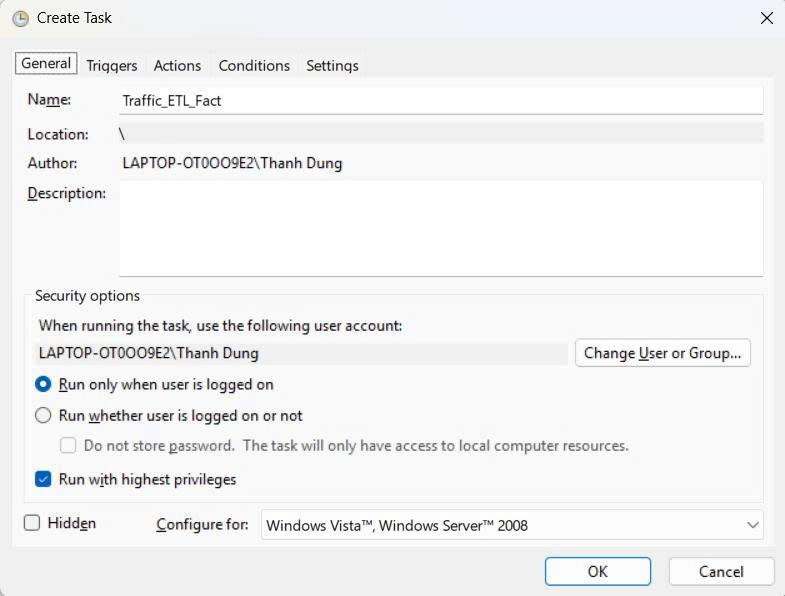
\includegraphics[width=0.8\textwidth]{Images/ETL_24}
    \vspace{6mm}
    \caption{Giao diện Task Scheduler}
    \label{fig:etl_24}
\end{figure}

\paragraph{ Xử lý nạp dữ liệu Tác động Thời tiết (Fact Weather Impact ETL)}

Module \texttt{etl/fact/etls\_fact\_weather\_impact.py} được thiết kế để thực hiện các phép phân tích phái sinh nhằm định lượng hóa mức độ ảnh hưởng của thời tiết lên năng lực vận hành và độ an toàn của từng đoạn đường.

\begin{description}
    \item[A. Thuật toán tính toán chỉ số rủi ro (Risk Scoring Algorithm)] \hfill \\
    Hệ thống triển khai các mô hình toán học để chuyển đổi đơn vị vật lý thành thang điểm rủi ro từ 0 đến 100:
    \begin{itemize}
        \item \textbf{Chỉ số rủi ro ngập lụt (\textit{Flood\_Risk\_Score}):} Tính toán dựa trên lượng mưa tức thời ($P_{1h}$), hệ số tác động địa hình ($I_{factor}$) và năng lực thoát nước ($D_{capacity}$):
        \begin{equation}
            Flood\_Risk = \min \left( 100, \frac{P_{1h} \times I_{factor}}{D_{capacity}} \times 100 \right)
        \end{equation}
        \item \textbf{Chỉ số an toàn tầm nhìn (\textit{Visibility\_Safety\_Score}):} Đánh giá dựa trên trường \texttt{visibility}. Tầm nhìn dưới 500m kích hoạt cảnh báo nguy hiểm (\texttt{Danger}), trong khi tầm nhìn trên 2000m được coi là an toàn.
    \end{itemize}

    \item[B. Logic đối khớp không gian và làm giàu dữ liệu] \hfill \\
    Dữ liệu tác động thời tiết được gắn trực tiếp vào \texttt{segment\_key} dựa trên tọa độ trung tâm, cho phép nhận diện các "điểm đen" về ngập lụt trên từng con phố cụ thể. Đồng thời, hệ thống sử dụng bộ quy tắc logic (\texttt{Knowledge Base}) để suy diễn trạng thái mặt đường (Khô ráo, Trơn trượt, Ngập nước) dựa trên mã thời tiết.

    \item[C. Ý nghĩa đối với bài toán phân tích đa chiều] \hfill \\
    Cho phép thực hiện phép \texttt{JOIN} giữa \texttt{fact\_traffic\_flow} và \texttt{fact\_weather\_impact} để tìm ra hệ số giảm tốc độ trung bình của xe máy khi trời mưa, cung cấp dữ liệu nền tảng cho các thuật toán dự báo tắc nghẽn.
\end{description}

\begin{figure}[htbp]
    \centering
    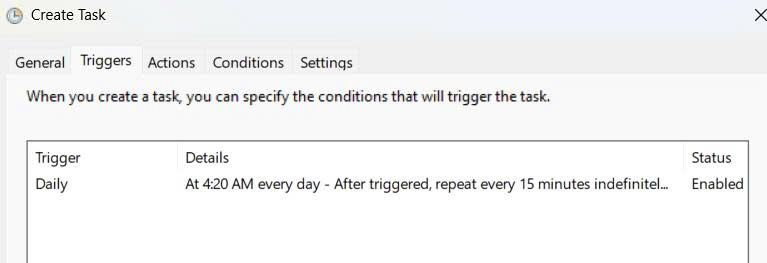
\includegraphics[width=0.5\textwidth]{Images/ETL_25}
    \vspace{6mm}
    \caption{Set up Trigger theo lịch ETL}
    \label{fig:etl_25}
\end{figure}
\subsubsection{ Quy trình giả lập dữ liệu (Mock Data Pipeline)}

Trong giai đoạn phát triển và tối ưu hóa kho dữ liệu, việc chỉ phụ thuộc vào dữ liệu thời gian thực từ API là chưa đủ để kiểm chứng các mô hình phân tích dài hạn hoặc kiểm thử hiệu năng truy vấn trên quy mô lớn. Do đó, hệ thống triển khai một Pipeline chuyên biệt để giả lập dữ liệu (Mock Data) thông qua module \texttt{pipelines/run\_all\_mocks.py}. Quy trình này mô phỏng các thực thể người dùng, hành vi di chuyển và hiệu suất hạ tầng dựa trên các quy luật xác suất thực tế.

\paragraph{ Giả lập thực thể Người dùng (User Mocking)}

Module \texttt{etl/mock/etl\_mock\_user.py} thực hiện khởi tạo tập khách hàng giả lập cho hệ thống:
\begin{itemize}
    \item \textbf{Tạo dữ liệu định danh:} Sử dụng thư viện \texttt{Faker} để sinh ra các thông tin như tên người dùng, số điện thoại và email đảm bảo tính duy nhất và định dạng chuẩn.
    \item \textbf{Quản lý trạng thái:} Mỗi người dùng được gán các thuộc tính như ngày đăng ký (\texttt{created\_at}) lùi về quá khứ để tạo ra tập dữ liệu có chiều sâu thời gian, phục vụ cho các báo cáo về tăng trưởng người dùng (User Growth).
    \item \textbf{Nạp dữ liệu:} Toàn bộ dữ liệu được đẩy vào bảng \texttt{dim\_user} thông qua kỹ thuật \texttt{Batch Insert} để tối ưu tốc độ.
\end{itemize}

\paragraph{ Mô phỏng hành trình di chuyển (Trip Mocking)}

Đây là phần phức tạp nhất trong quy trình giả lập, thực hiện tại \texttt{etl/mock/etl\_mock\_trip.py} để nạp dữ liệu vào bảng \texttt{fact\_trip}:
\begin{itemize}
    \item \textbf{Logic chọn lộ trình:} Hệ thống thực hiện lấy ngẫu nhiên các cặp \texttt{segment\_key} từ bảng \texttt{dim\_segment} để làm điểm bắt đầu và điểm kết thúc của một chuyến đi.
    \item \textbf{Tính toán thông số chuyến đi:}
    \begin{itemize}
        \item \textbf{Khoảng cách ($d$):} Được tính toán dựa trên độ dài thực tế của các phân đoạn đường được chọn.
        \item \textbf{Thời gian di chuyển ($t$):} Được suy diễn từ vận tốc trung bình của loại xe (\texttt{avg\_speed} trong \texttt{dim\_vehicle\_type}) cộng thêm một sai số ngẫu nhiên (\textit{Random Variance}) để mô phỏng tình trạng giao thông biến động.
    \end{itemize}
    \item \textbf{Tiêu hao nhiên liệu và Khí thải:} Hệ thống áp dụng các công thức ước tính để sinh dữ liệu cho cột \texttt{fuel\_consumed\_liters} và \texttt{co2\_emitted\_kg}, hỗ trợ cho các bài toán phân tích môi trường.
\end{itemize}

\paragraph{ Giả lập Hiệu suất Phân đoạn lịch sử (Segment Performance Mocking)}

Để Dashboard có thể hiển thị các biểu đồ so sánh theo năm/tháng, module \texttt{etl/mock/etl\_mock\_segment\_performance.py} thực hiện nạp dữ liệu lịch sử giả định cho bảng \texttt{fact\_segment\_performance}:
\begin{itemize}
    \item \textbf{Tạo dữ liệu Baseline:} Hệ thống lấy dữ liệu vận tốc thiết kế từ \texttt{dim\_way} làm mốc chuẩn.
    \item \textbf{Mô phỏng chu kỳ thời gian:} Dữ liệu được sinh ra theo quy luật: giảm tốc độ vào các khung giờ cao điểm (Morning/Afternoon Shifts) và tăng tốc độ vào ban đêm.
    \item \textbf{Lợi ích:} Việc này giúp kiểm thử tính đúng đắn của các câu lệnh SQL Aggregate phức tạp trước khi có đủ dữ liệu thực tế sau nhiều tháng vận hành.
\end{itemize}

\subsection{TỰ ĐỘNG HÓA VÀ GIÁM SÁT VẬN HÀNH (AUTOMATION \& MONITORING)}

Để đảm bảo kho dữ liệu luôn phản ánh trạng thái mới nhất của mạng lưới giao thông mà không cần sự can thiệp thủ công từ quản trị viên, dự án đã triển khai một hệ thống vận hành tự động hóa hoàn toàn. Cơ chế này chuyển đổi các kịch bản xử lý dữ liệu đơn lẻ thành một chu kỳ sống liên tục, đáp ứng tiêu chuẩn của một hệ thống Real-time Data Warehouse.

\subsubsection{ Cơ chế vận hành thông qua Batch Script và Điều phối hệ thống}

Tệp kịch bản \texttt{scripts/run\_etl\_fact\_daily.bat} đóng vai trò là lớp vỏ điều phối (\textit{Wrapper}) bên ngoài, giúp kết nối mã nguồn Python với hệ điều hành Windows.

\paragraph{ Tự động hóa quản lý môi trường thực thi (Virtual Environment Activation)}

Batch script thực hiện kích hoạt môi trường cô lập bằng lệnh \texttt{call .venv\textbackslash Scripts\textbackslash activate}. Điều này đảm bảo rằng mọi thư viện quan trọng như \texttt{ultralytics}, \texttt{psycopg2} và \texttt{OSMnx} luôn được chạy đúng phiên bản đã kiểm thử, loại bỏ hoàn toàn các lỗi thiếu Module khi chạy tự động.

\begin{figure}[htbp]
\centering
\begin{minipage}{0.9\textwidth}
\begin{verbatim}
@echo off
setlocal enabledelayedexpansion
chcp 65001 > nul
cd /d "C:\Path\To\Project\project_folder"
if not exist "logs" mkdir "logs"
call .venv\Scripts\activate
echo [START] ETL JOB STARTED AT %TIME%
powershell -Command "python -u main_etl.py --mode fact 2>&1 | Tee-Object ..."
pause
\end{verbatim}
\end{minipage}
\vspace{6mm}
\caption{Cấu trúc tệp lệnh Batch thực thi chu kỳ ETL tự động}
\label{fig:etl_26}
\end{figure}

\paragraph{ Chiến lược lập lịch chu kỳ (Windows Task Scheduler Integration)}

Dự án tận dụng Windows Task Scheduler làm "nhịp đập" cho toàn hệ thống với tần suất thực thi 15 phút một lần. Đây là khoảng thời gian tối ưu để cân bằng giữa độ trễ dữ liệu và hạn mức API miễn phí. Cấu hình "Run whether user is logged on or not" đảm bảo quy trình ETL vẫn diễn ra ngầm định ngay cả khi không có người dùng đăng nhập.

\paragraph{ Tối ưu hóa tham số và Quản lý tài nguyên}

Việc sử dụng tham số \texttt{--mode fact} giúp hệ thống chỉ tập trung vào các bảng dữ liệu biến động, giảm thời gian thực thi mỗi Batch xuống dưới 3 phút, từ đó giải phóng tài nguyên CPU/GPU cho các tác vụ khác.

\subsubsection{ Hệ thống ghi nhật ký tập trung (Logging System)}

Hệ thống triển khai cơ chế \textit{Centralized Logging} dựa trên thư viện \texttt{logging} tiêu chuẩn của Python.

\begin{itemize}
    \item \textbf{Tiêu chuẩn hóa cấu trúc nhật ký:} Sử dụng định dạng \texttt{[Thời gian] - [Tên Module] - [Cấp độ] - [Thông điệp]}. Nhật ký được ghi song song ra màn hình console và tệp tin \texttt{.log} để phục vụ tra cứu.
    \item \textbf{Giám sát sức khỏe Pipeline (Health Monitoring):} Nhật ký ghi lại chi tiết số lượng bản ghi nạp thành công, số lượng bị lỗi (\textit{Skip}) và tổng thời gian thực thi, giúp đánh giá độ bao phủ dữ liệu (\textit{Data Coverage}).
    \item \textbf{Quản lý ngoại lệ (Exception Handling):} Hệ thống bắt các ngoại lệ cụ thể (như \texttt{psycopg2.Error}) và ghi lại \textit{Error Traceback}, giúp quản trị viên phân biệt lỗi do hạ tầng hay lỗi từ API bên thứ ba.
\end{itemize}

\begin{figure}[htbp]
    \centering
    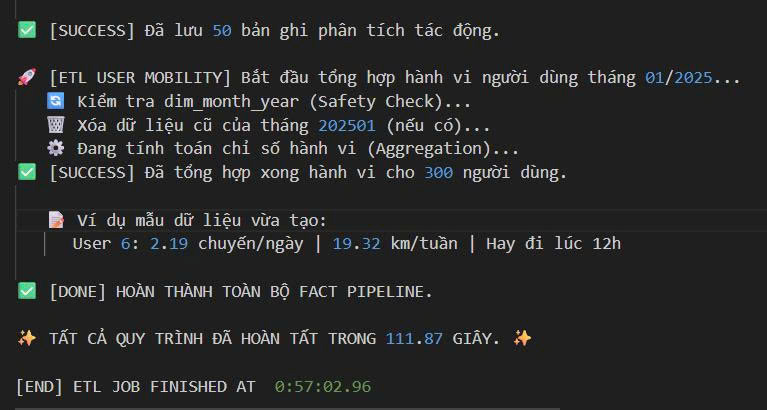
\includegraphics[width=0.9\textwidth]{Images/ETL_27}
    \vspace{6mm}
    \caption{Nhật ký tổng hợp kết thúc quy trình Fact Pipeline thành công}
    \label{fig:etl_27}
\end{figure}

\subsection{Kết chương}

Chương 8 đã trình bày một cách toàn diện quy trình xây dựng hệ thống ETL – trung tâm điều phối của kho dữ liệu giao thông thông minh. Chương này đã đạt được các kết quả kỹ thuật then chốt:

\begin{itemize}
    \item \textbf{Kiến trúc đa tầng bền vững:} Hiện thực hóa mô hình điều phối từ \texttt{main\_etl.py} đến các pipeline nguyên tử, tối ưu hóa tài nguyên và quản lý lỗi tập trung.
    \item \textbf{Chuẩn hóa Không gian - Thời gian:} Giải quyết thành công bài toán tích hợp dữ liệu GIS, tự động hóa phân đoạn đường và xử lý lịch âm cho ngày lễ Việt Nam.
    \item \textbf{Hợp nhất dữ liệu AI:} Tích hợp thành công mô hình \textbf{YOLOv8} để thu thập lưu lượng xe quy đổi PCU, kết hợp cùng API vận tốc và thời tiết.
    \item \textbf{Vận hành tự động:} Thiết lập cơ chế chạy định kỳ qua Batch Script và Task Scheduler, đảm bảo kho dữ liệu tự vận hành ổn định 24/7.
\end{itemize}

Kết quả của Chương 8 là một nền tảng dữ liệu sạch và giàu ngữ cảnh, sẵn sàng cho việc xây dựng Dashboard và các mô hình phân tích nâng cao ở chương kế tiếp.